% debut d'un fichier latex standard
\documentclass[a4paper,12pt,twoside]{article}

% pour l'inclusion de figures en eps,pdf,jpg
\usepackage{graphicx}
\usepackage{subcaption}
\usepackage{wrapfig}
% quelques symboles mathematiques en plus
\usepackage{amsmath}
% le tout en langue francaise
%\usepackage[french]{babel}
% on peut ecrire directement les caracteres avec l'accent
% a utiliser sur Linux/Windows
\usepackage[utf8]{inputenc}
\usepackage[T1]{fontenc}
% a utiliser sur le Mac
%\usepackage[applemac]{inputenc}
% pour l'inclusion de links dans le document
\usepackage[colorlinks,bookmarks=false,linkcolor=blue,urlcolor=blue]{hyperref}
\usepackage{siunitx}

\paperheight=297mm
\paperwidth=210mm

\setlength{\textheight}{235mm}
\setlength{\topmargin}{-1.2cm} % pour centrer la page verticalement
%\setlength{\footskip}{5mm}
\setlength{\textwidth}{15cm}
\setlength{\oddsidemargin}{0.56cm}
\setlength{\evensidemargin}{0.56cm}

\pagestyle{plain}

% quelques abreviations utiles
\def \be {\begin{equation}}
\def \ee {\end{equation}}
\def \dd  {{\rm d}}

\newcommand{\mail}[1]{{\href{mailto:#1}{#1}}}
\newcommand{\ftplink}[1]{{\href{ftp://#1}{#1}}}
%
% latex SqueletteRapport.tex      % compile la source LaTeX
% xdvi SqueletteRapport.dvi &     % visualise le resultat
% dvips -t a4 -o SqueletteRapport.ps SqueletteRapport % produit un PostScript
% ps2pdf SqueletteRapport.ps      % convertit en pdf

% pdflatex SqueletteRapport.pdf    % compile et produit un pdf

% ======= Le document commence ici ======

\begin{document}
% Le titre, l'auteur et la date
\title{Gravitational systems.\\{\small Apollo 13, atmosphere re-entry and Trojan asteroids \\ Physique Numérique I}\\{\small Rapport 4}}
\date{\today}
\author{Delphine Martres et Damien Korber\\{\small \mail{delphine.martres@epfl.ch} et \mail{damien.korber@epfl.ch}}}
\maketitle
\tableofcontents % Table des matieres

% Quelques options pour les espacements entre lignes, l'identation
% des nouveaux paragraphes, et l'espacement entre paragraphes
\baselineskip=16pt
\parindent=15pt
\parskip=5pt
\newpage


%%%% ON COMMENCE A ECRIRE D'ICI

\section{Introduction}

\section{"Houston, we've had a problem"}
Apollo 13 is located at a distance $r_0 = \SI{314159}{\kilo\meter}$ from the center of Earth.
Its velocity with respect to earth's frame of reference is $v_0 = \SI{1.2}{\kilo\meter\per\second}$.
Because of a fuel shortage, the norm of speed can not be changed.
However, it is possible to ajust its direction.
To bring back Apollo 13's crew, their trajectory needs to get as close as $h=\SI{10}{\kilo\meter}$ to the surface of earth, the distance where the atmosphere is dense enough to slow the ship and break its orbit.
In this experiment, the Moon will be ignored and the mass of Apollo 13 is neglictable compared to Earth's mass. Then, it will be a 1 body gravitationnal problem.
%TODO : Est-ce qu'il faut mettre là toutes les constantes ? Y'en a plein et je les définis quand on en a besoin...

\subsection{Initial velocity of Apollo 13}
The goal of this section is to find the componants of the velocity of the probs, so that it get close to earth, at \SI{10}{\kilo\meter}.
Two physical laws are considered to solve this problem. %TODO : C'est pas des lois, t'as un autre mot ?
\begin{itemize}
  \item Conservation of mechanical energy
  \item Conservation of angular momentum
\end{itemize}

\subsubsection{Conservation of mechanical energy}
The mechanical energy of the probe at any moment is given by equation \eqref{eq:1a-em-apollo13}.
\begin{equation}
  E_m = \frac{1}{2}mv^2 - G\frac{mM}{r}
  \label{eq:1a-em-apollo13}
\end{equation}
where $m=\SI{5809}{\kilo\gram}$ is the mass of the probe, $M=\SI{5.972d24}{\kilo\gram}$ is the mass of earth, $G=\SI{6.674d-11}{\cubic\meter\per\kilo\gram\per\square\second}$ is the gravitational constant, $v$ is the speed of the probe with respect to earth's frame of reference, and $r$ is the distance between the probe and the center of earth.\\

By conservation of mechanical energy, two moments are chosen.
\begin{itemize}
  \item $t=\SI{0}{\s}: E_{m,t_0} = \frac{1}{2}mv_0^2 - G\frac{mM}{r_0}$
  \item $t=t_{end}: E_{m,t_{end}} = \frac{1}{2}mv_{end}^2 - G\frac{mM}{h + R_t}$
\end{itemize}
where $v_0 = \SI{1.2}{\kilo\meter\per\second}$ is the initial velocity of Apollo 13, $r_0 = \SI{314159}{\kilo\meter}$ is the initial distance between Apollo 13 and the center of earth.
Thus, solving $E_{m,t_0} = E_{m,t_{end}}$, the velocity of the probe when it is at a distance $h=\SI{10}{\kilo\meter}$ of earth can be found, and is given by equation \eqref{eq:1a-vitesse-finale}.

\begin{equation}
  v_{end} = \sqrt{v_0^2 + 2GM\left(\frac{1}{h + R_t} - \frac{1}{r_0}\right)}
  \label{eq:1a-vitesse-finale}
\end{equation}

\subsubsection{Conservation of angular momentum}
%TODO : À écrire.

\subsubsection{Maximum velocity of the probe}
The maximum velocity of the probe on this given situation is given by equation \eqref{eq:1a-vitesse-finale}.
This affirmations comes from the fact that, as the gravitational force is the only one considered, the maximum velocity is given by the moment where the distance is minimal, which is $h_{min}$ in this situation.
Thus, after some computation, the maximum velocity reached by Apollo 13 is given by equation \eqref{eq:1a-vitesse-max}.

\begin{equation}
  v_{max} = \SI{11121.52}{\meter\per\second} %TODO : Donnée à verifier, elle n'est peut-être pas à jour. (calculs.nb)
  \label{eq:1a-vitesse-max}
\end{equation}




\subsection{Numerical analysis with a non-adaptative time step}
In this section, the simulation of the previous simulation will be computed numerically, using the numerical method: Runge-Kutta of order 4 (RK4).

\subsubsection{Trajectory}
The trajectory of Apollo 13 and earth are represented in figure \ref{fig:1b-trajectory-non-adaptative}.
In this figure, earth is considered circular and is drawn at the right scale.
The green cross represents the initial position of Apollo 13, and the green points are its trajectory.

\begin{figure}[h]
  \centering
  \includegraphics[width=0.5\textwidth]{graphs/ex1b-traj.eps}
  \caption{blabla}
  \label{fig:1b-trajectory-non-adaptative}
\end{figure}

%TODO : Un peu d'analyse de la trajectoire

\subsubsection{Convergence studies: $h_{min}$ and $v_{max}$}
To study the convergence of RK4, the minimal distance between Earth's surface and Apollo 13, and the maximal speed of Apollo 13 will be studied.
The convergence studies are represented in figure \ref{fig:1b_conv}.

\begin{figure}[h]
  \centering
  \begin{subfigure}[t]{0.45\textwidth}
    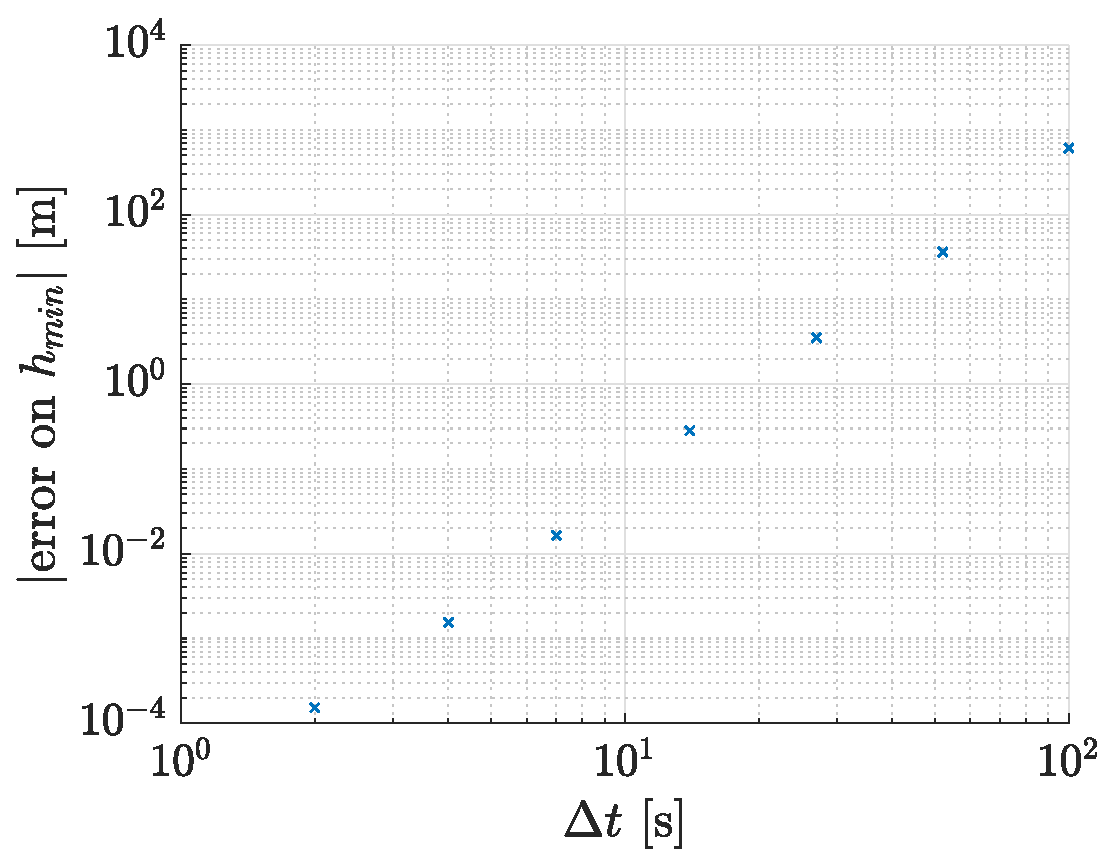
\includegraphics[width=\textwidth]{graphs/ex1b_conv_h.eps}
    \caption{blabla}
    \label{fig:1b_conv_hmin}
  \end{subfigure}
  ~
  \begin{subfigure}[t]{0.45\textwidth}
    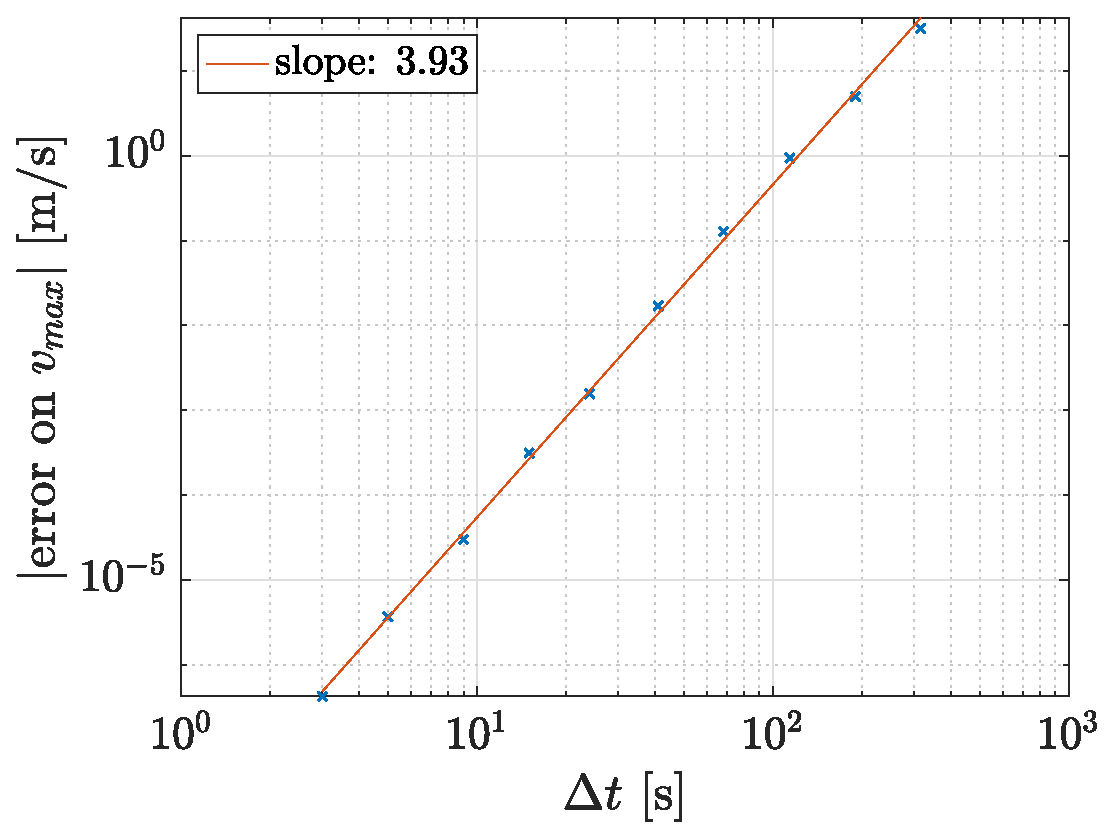
\includegraphics[width=\textwidth]{graphs/ex1b_conv_vel.eps}
    \caption{blabla}
    \label{fig:1b_conv_vmax}
  \end{subfigure}
  \caption{blabla}
  \label{fig:1b_conv}
\end{figure}

%TODO : Analyser ces graphs.

\subsection{Numerical analysis with an adaptative time step}
This time, the same sitation is computed numerically, but with an adaptative time step.
It means that, for each steps, the time step is adapted to reach a particular precision.
It allows to use greater time steps when the evolution is slightly changing, and to use smaller time steps when the evolution is greatly changing.
Thus, it greatly reduces the number of steps required to do a simulation.

\subsubsection{Convergence study on the precision}
The adaptative time step is controlled by a factor, $\epsilon$, which provides the precision that the next step has to reach.
By varying $\epsilon$, the convergence of $h_{min}$ with respect to the number of steps can be studied.
The resulting study is represented in figure \ref{fig:1c-conv-epsilon}.

\begin{figure}[h]
  \centering
  \includegraphics[width=0.5\textwidth]{graphs/ex1c-conv-epsilon.eps}
  \caption{blabla}
  \label{fig:1c-conv-epsilon}
\end{figure}

%TODO : Analyser ce graph.

Figure \ref{fig:1c-dt} represents the evolution of dt over time for one simulation.

\begin{figure}[h]
  \centering
  \includegraphics[width=0.5\textwidth]{graphs/ex1c-dt.eps}
  \caption{blabla}
  \label{fig:1c-dt}
\end{figure}

%TODO : Parler plus en profondeur de ce graph.

\section{"Houston, we're going to have a real problem"}
\subsection{PARTIE A - CHANGER TITRE}

\subsection{Rotating the probe to get the minimal acceleration}
This section will focus on a way to minimize the acceleration underwent by the astronauts in Apollo 13.

The method is quite simple: slightly changing the direction of the initial velocity of the probe.
To achieve this, the initial velocity will be rotated by an angle $\theta$ that will be found in an empirical way.
Note that the probe must land on its first entry in the atmosphere: it should not slow with multiples periods around earth. %TODO : Je trouve cette phrase pas très belle.

Let $\mathbf{v} = \begin{pmatrix} v_1, v_2\end{pmatrix}$ be the initial velocity and $\mathbf{w} = \begin{pmatrix} w_1, w_2\end{pmatrix}$ be the rotated initial velocity.
Both velocities are linked by the rotation matrix, and their relation is given by equation \eqref{eq:v-rotation}.

\begin{equation}
  \begin{pmatrix}
    w_1 \\
    w_2
  \end{pmatrix}
  =
  \begin{pmatrix}
    \cos\theta & -\sin\theta \\
    \sin\theta & \cos\theta
  \end{pmatrix}
  \begin{pmatrix}
    v_1 \\
    v_2 \\
  \end{pmatrix}
  =
  \begin{pmatrix}
    v_1\cos\theta - v_2\sin\theta \\
    v_1\sin\theta + v_2\cos\theta
  \end{pmatrix}
  \label{eq:v-rotation}
\end{equation}

To find the right angle $\theta$ minimizing the acceleration, the plot of the maximum acceleration for a given angle, and the trajectory of the probe, will be use.

Denote $i$ the process number, $\phi_0$ an arbitrary angle and $\Theta_0 = 0$ an angle.
First, an arbitrary range of angles are selected: $A_0 = [\Theta_0-\phi_0, \Theta_0+\phi_0]$.
The rotated velocities $\mathbf{w}$ are computed and stored, for $N$ angles contained in $A$.
These velocities are inserted as the initial velocities, and all the simulations are made.
Next, the two plot cited above are created and analysed.
The plot of trajectory gives an idea of the angles to ignore (those where the probe does not land on the period).
Regarding the left angles, the plot of maximum acceleration gives the best angle in this range, the one giving the smallest maximum acceleration. This angle is denoted by $\Theta_1$.
The process is restarted with a new range of angles $A_1 = [\Theta_1 - \phi_1, \Theta_1 + \phi_1]$, where $\phi_1 < \phi_0$.
By looping $k$ times, until the moment where the minimal acceleration only slightly changes over analysis,  one of the best angle is found.
This angle is given by $\theta = \Theta_k$.

To illustate this method, figure \ref{fig:2b-min-a} gives an example of the plots that can be made for one process.

\begin{figure}[h]
  \centering
  \begin{subfigure}[t]{0.45\textwidth}
    \includegraphics[width=\textwidth]{graphs/2b-min-a-traj.eps}
    \caption{blabla}
    \label{fig:2b-min-a-traj}
  \end{subfigure}
  ~
  \begin{subfigure}[t]{0.45\textwidth}
    \includegraphics[width=\textwidth]{graphs/2b-min-a-comp.eps}
    \caption{blabla}
    \label{fig:2b-min-a-comp}
  \end{subfigure}
  \caption{blabla}
  \label{fig:2b-min-a}
\end{figure}

The angle of rotation found using this processes is given by equation \eqref{eq:2b-a-min-angle}.

\begin{equation}
  \theta = XXX\SI{}{\radian} %TODO : Compléter ce résultat.
  \label{eq:2b-a-min-angle}
\end{equation}

The norm of the smallest maximal acceleration, found using angle of equation \eqref{eq:2b-a-min-angle}, is given by equation \eqref{eq:2b-a-min}.

\begin{equation}
  a = XXX\SI{}{\meter\per\square\second} = XXX\num{}\text{G} %TODO : Compléter ce résultat.
  \label{eq:2b-a-min}
\end{equation}

%TODO : Peut-être qu'il faut mettre ces résultat en inline, parce que ça prend beaucoup de place pour pas beaucoup de visibilité de mettre ça en équation.

\section{Two bodies: Earth and Moon}

\section{Three bodies: Earth, Moon and Apollo 13}

\section{Three bodies: Earth, Moon and a third body - Lagrangian points}






\end{document}
